\documentclass[a4paper,11pt]{article}
\usepackage{indentfirst}
\usepackage[T1]{fontenc}
\usepackage[polish]{babel}
\usepackage[utf8]{inputenc}
\usepackage{lmodern}
\selectlanguage{polish}
\usepackage[top=2cm, bottom=2cm, left=1cm, right=1cm]{geometry}
\usepackage{lastpage}
\usepackage{fancyhdr}
\pagestyle{fancy}
\setlength\parindent{24pt}
\makeatletter
\newcommand{\linia}{\rule{\linewidth}{0.4mm}}
\renewcommand{\maketitle}{\begin{titlepage}
    \vspace*{2cm}
    \begin{center}\LARGE
    Politechnika Warszawska\\
    Wydział Elektryczny\\
    \end{center}
    \vspace{5cm}
    \noindent\linia
    \begin{center}
      \LARGE \textsc{\@title}
         \end{center}
     \linia
    \vspace{0.5cm}
    \begin{flushright}
    \begin{minipage}{5cm}
    \textit{Autor:}\\
    \normalsize \textsc{\@author} \par
    \end{minipage}
    \vspace{5cm}
     \end{flushright}
    \vspace*{\stretch{6}}
    \begin{center}
    \@date
    \end{center}
  \end{titlepage}
}
\makeatother
\author{Grzegorz Kopyt \\ Arkadiusz Michalak}
\title{Specyfikacja Funkcjonalna\\Projekt Zespołowy 2018/2019}
\usepackage{graphicx}

\fancyhf{}
\rfoot{\thepage{}/\pageref{LastPage}}

\begin{document}
\maketitle

\tableofcontents
\vspace{1cm}
\noindent\linia
\section{Wstęp teoretyczny}
Dokument ten dotyczy programu realizowanego w ramach ,,Projektu Zespołowego 2018/2019".

Głównym zadaniem jest analiza i podział terenu na optymalne części. Program na podstawie podanego konturu terenu oraz punktów kluczowych, znajdujących się na tym terenie, powinien podzielić go na optymalne części. Oznacza to, że każdy z powstałych obszarów powinien zawierać jeden punkt kluczowy, a granice powinny obejmować każde miejsce, z którego bliżej jest do danego punktu kluczowego niż do jakiegokolwiek innego z~punktów kluczowych.

Dodatkowo na całą mapę zostaną naniesione różne typy obiektów (między innymi domy z mieszkańcami), a~program powinien przygotować statystykę ilości obiektów oraz mieszkańców na danej części terenu.

Ważnym założeniem jest to, że pod danymi współrzędnymi może znajdować się tylko jeden punkt kluczowy lub obiekt.

Pozostałe funkcje programu zostały opisane w sekcji ,,Wymagania funkcjonalne".

\noindent\linia
\section{Wymagania funkcjonalne}

Program powinien spełniać podane wymagania funkcjonalne:
\begin{itemize}
\item podanie danych z pliku:
\begin{itemize}
\item podanie konturu terenu,
\item podanie rozmieszczeniem punktów kluczowych,
\item podawanie obiektów i definiowanie ich typów.
\end{itemize}
\item analiza terenu:
\begin{itemize}
\item podzielenie terenu na optymalne obszary,
\item wyświetlanie listy obiektów należących do danego obszaru,
\item wyświetlanie zbiorcze listy obiektów należących do danego obszaru,
\item wyświetlanie liczby mieszkańców danego obszaru.
\end{itemize}
\item wizualizacja:
\begin{itemize}
\item narysowanie granic optymalnych obszarów,
\item naniesienie na wczytany teren obiektów.
\end{itemize}
\item modyfikacja po wprowadzeniu danych z pliku:
\begin{itemize}
\item dodawanie i usuwanie elementów konturu terenu,
\item dodawanie i usuwanie punktów kluczowych,
\item nakładanie grafiki pod wyznaczone kontury.
\end{itemize}
\end{itemize}

Plik wejściowy powinien być zgodny z podanym wzorem:

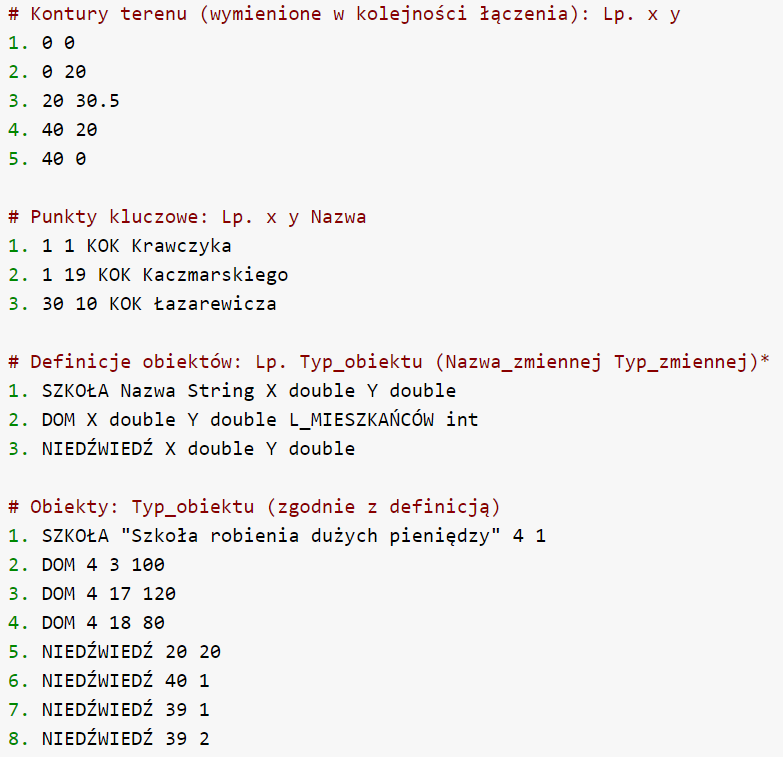
\includegraphics[scale=0.70]{ExampleInputFile}

Uwagi:
\begin{itemize}
\item kolejne sekcje pliku powinny być oddzielane znakiem \textit{\#};
\item obsługiwane typy możliwe do użycia przy definicji nowych typów to: string, int, double;
\item wartości zmiennych typu string powinny być podane w cudzysłowie;
\item nazwy obiektów powinny być bez spacji i zawierać do 40 znaków;
\item podane punkty kluczowe i obiekty muszą znajdować się wewnątrz podanego konturu terenu lub na jego krawędzi;
\item jeśli podany kontur będzie otwarty, ostatni jego punkt zostanie połączony z pierwszym;
\item podany kontur musi być figurą wypukłą;
\item krawędzie konturu terenu nie mogą się przecinać;
\item muszą zostać podane obiekty \textit{DOM}, \textit{NIEDŹWIEDŹ}, \textit{SZKOŁA} wraz z ich definicjami, takimi jak w pliku przykładowym;
\item plik musi być kodowany w UTF-8.
\end{itemize}
\noindent\linia
\section{Obsługa}
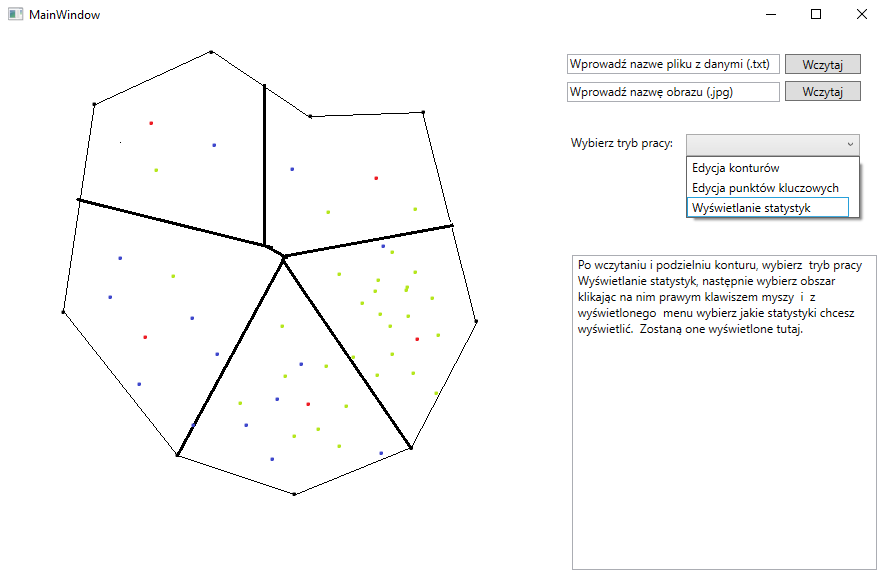
\includegraphics[scale=0.75]{GUI_EXAMPLE.png}

Uruchomienie programu:
\begin{itemize}
\item po uruchomieniu programu należy wybrać plik danych. Po kliknięciu klawisza wyświetli się okno przeglądania plików, wzorzec pliku wejściowego znajduje się w \textbf{rozdziale 2},
\item opcjonalnie można wczytać obraz tła korzystając z odpowiedniego przycisku, wyświetla się okno przeglądania plików.
\end{itemize}
Tryb edycji konturów:
\begin{itemize}
\item po wybraniu tego trybu pracy użytkownik zyskuje możliwość zmiany wyglądu konturów analizowanego obszaru,
\item po wybraniu prawym przyciskiem myszy punktu konturu wyświetli się menu, punkt można usunąć, wtedy punty do niego sąsiednie zostaną połączone, można go również przesunąć zachowując obecne połączenie,
\item po wybraniu prawym przyciskiem linii konturu można dodać nowy punkt który zostanie połączony z punktami wyznaczającymi daną linie, a wybrana linia zostanie usunięta.
\end{itemize}
Tryb edycji punktów kluczowych:
\begin{itemize}
\item po wybraniu tego trybu pracy użytkownik może manipulować punktami kluczowymi,
\item po wybraniu punktu prawym przyciskiem myszy wyświetli się menu, plik można usunąć lub przenieść go w inne miejsce,
\item w dowolnym pustym miejscu w konturze po kliknięciu prawym przyciskiem myszy pojawi się możliwość dodania nowego punktu kluczowego.
\end{itemize}
\pagebreak
Tryb wyświetlania statystyk:
\begin{itemize}
\item sposób działania najważniejszego dla użytkownika trybu zostanie zawarty w interfejsie graficznym programu,
\item po wybraniu obszaru prawym przyciskiem myszy menu pozwoli określić jakie statystyki użytkownik chce wyświetlić w przygotowanym do tego oknie:
\begin{itemize}
\item lista obiektów należących do obszaru,
\item pogrupowana typami lista obiektów,
\item liczba mieszkańców danego obszaru.
\end{itemize}
\end{itemize}
\noindent\linia
\section{Komunikaty o błędach}
W przypadku wystąpienia błędu pojawi się okno z komunikatem o tym błędzie.

Przykładowe komunikaty wyglądają następująco:
\begin{itemize}
\item nie podano pliku wejściowego:

\textit{There was no file given.}
\item podano błędny plik wejściowy:

\textit{Incorrect file. Line 24 is wrong. Compare it with the file pattern and try again.}
\item podany plik nie jest kodowany w UTF-8:

\textit{Incorrect file. It is not created with UTF-8 encoding.}
\item podany kontur nie jest figurą wypukłą:

\textit{Incorrect file. The terrain contour is not a convex figure.}
\item podane krawędzie konturu przecinają się:

\textit{Incorrect file. Edges of the given contour are crossing. Fix it and try again.}
\item podany punkt kluczow nie zawiera się wewnątrz konturu:

\textit{Ignored key point (3,5). The given key point is out of bounds of the terrain contour.}
\item podany obiekt nie zawiera się wewnątrz konturu:

\textit{Ignored DOM (5,71). The given object is out of bounds of the terrain contour.}
\item podany obiekt duplikuje współrzędne innego obiektu lub punktu kluczowego:

\textit{Ignored DOM (2,39). The given object's coordinates are already used.}
\item podany punkt kluczowy duplikuje współrzędne innego obiektu lub punktu kluczowego:

\textit{Ignored key point (2,39). The given key point's coordinates are already used.}

\end{itemize}

\noindent\linia
\section{Testy akceptacyjne}
\begin{itemize}
\item wczytanie pliku zawierającego prostu kontur i kilka punktów kluczowych;
\item dodanie nowego punktu kluczowego w obszarze konturu;
\item próba dodania punktu kluczowego poza obszarem konturu;
\item próba dodania punktu kluczowego nad innym obiektem;
\item przesunięcie punktu wyznaczającego kontur w taki sposób, że krawędzie będą się przecinać;
\end{itemize}
Program będzie uznany za działający jeśli pozytywnie przejdzie wszystkie testy. Pod słowem pozytywnie rozumie się wyświetlenie rezultatów, lub odpowiedni komunikat błędu który pozwoli użytkownikowi naprawić błąd.
\noindent\linia

\end{document}



